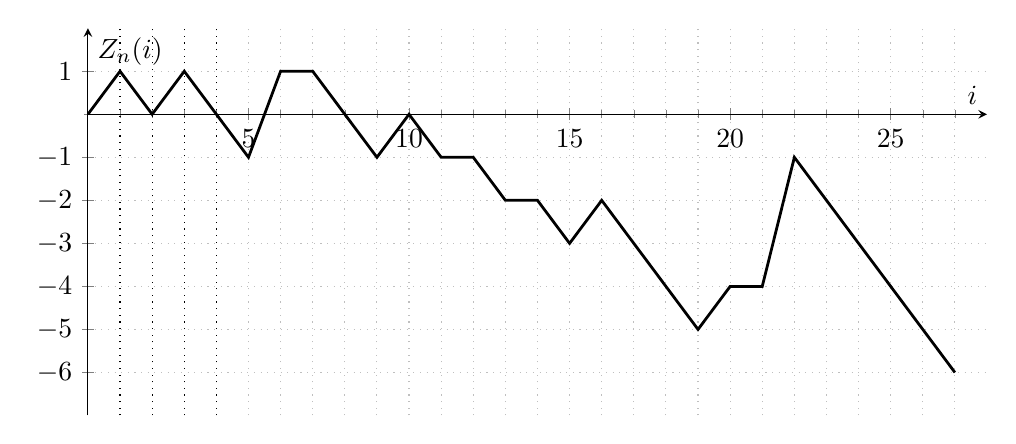
\begin{tikzpicture}
\begin{axis}[
axis x line=bottom,
axis y line=left,
grid = minor,
minor grid style={dotted},
xmin=0,
axis lines = middle,
xmax=28,
ymax = 2,
ymin  = -7,
xlabel={$i$},
ylabel={$Z_n(i)$},
xtick={5,10,15,20,25},
minor xtick = {1,...,27},
ytick={-6,...,1},
minor ytick={-6,...,1},
width = 13cm,
height = 6.5cm
]

\addplot [
line width=1.0pt
]
coordinates{
	(0,0) (1,1) (2,0) (3,1) (4,0) (5,-1)
	(6,1) (7,1) (8,0) (9,-1) (10,0) (11,-1) (12,-1) (13,-2) 
	(14,-2) (15,-3) 
	(16,-2) (17,-3) (18,-4) 
	(19,-5) 
	(20, -4) (21,-4) (22,-1) (23,-2) (24,-3) (25,-4) (26, -5) (27,-6)
};

\addplot [dotted] coordinates {(1, -7) (1, 2)};
\addplot [dotted] coordinates {(2, -7) (2, 2)};
\addplot [dotted] coordinates {(3, -7) (3, 2)};
\addplot [dotted] coordinates {(4, -7) (4, 2)};
\end{axis}

\end{tikzpicture} 